\begin{thm}{075}{\hosi ?}{}
 $\angle{A}$の二等分線上に点$B$を決め、線分$AB$を弦とする任意の円を描く。このとき、$AP+AQ$の長さは円の大きさによらず一定となることを示せ。
 \begin{center}
  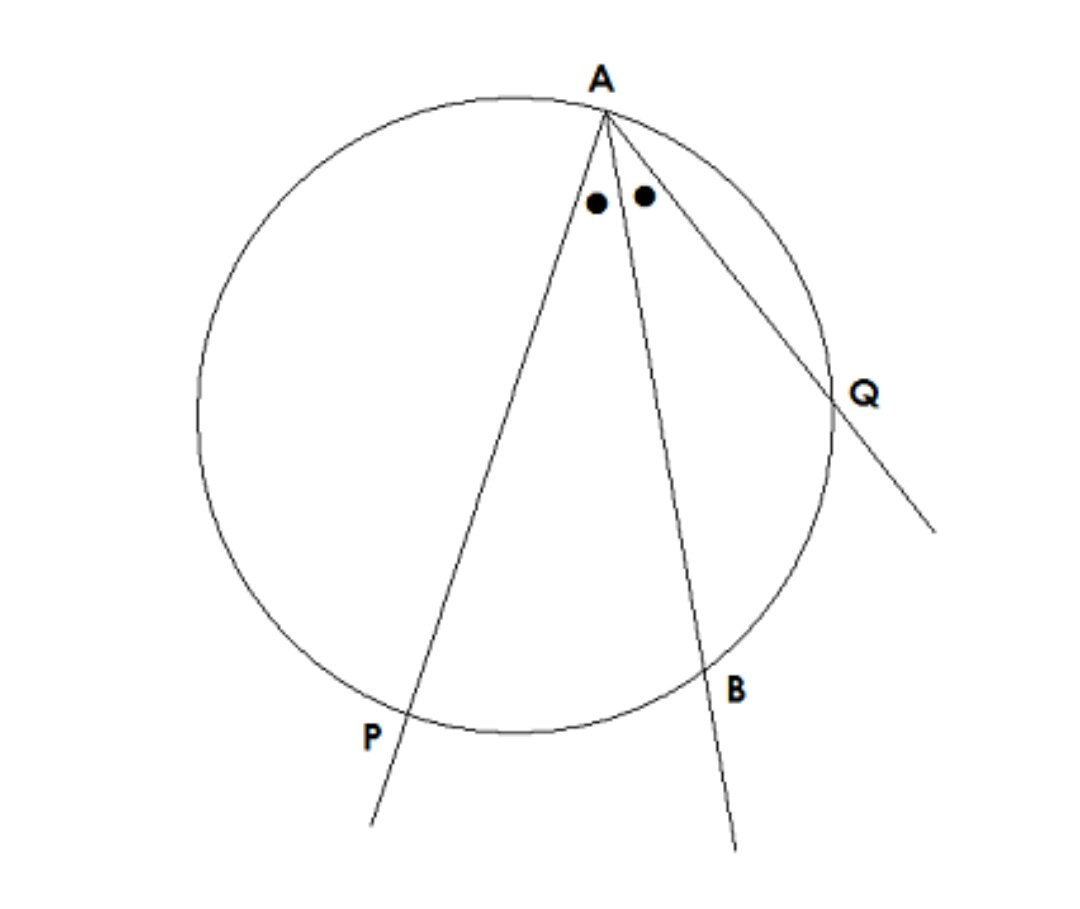
\includegraphics[bb=0 0 1080 909,width=0.9\linewidth]{../problems/Q_075/Q_075.jpg}
 \end{center}
\end{thm}

ここに解答を記述。